\chapter[Referencial teórico]{Referencial teórico}
\label{cap_Referencial teorico}
    
    No presente capítulo, serão discutidas as teorias e trabalhos relacionados a essa pesquisa. Primeiramente, será feita uma breve revisão quanto aos conceitos que sustentam a teoria da pesquisa. Posteriormente serão discutidos os trabalhos relacionados, indicando os pontos principais e as lacunas de estudo identificadas.  
    
    Sendo assim, com o intuito de levantar as informações citadas e identificar quais são as tecnologias de baixo custo que podem ser empregadas para obtenção das dimensões de bagagens, foi realizada uma revisão sistemática. Para tanto, foram definidas questões de pesquisa cuja revisão buscou responder, sendo elas:
    
    \begin{itemize}
        \item Quais são as tecnologias que podem servir para detectar a dimensão de bagagens?
        \item As tecnologias conseguem analisar bagagens com formatos não retangulares?
        \item As tecnologias conseguem analisar múltiplas bagagens (ex. uma em cima da outra)?
        \item A exatidão das tecnologias é sensível ao posicionamento da bagagem?
    \end{itemize}
    
%\section{Protocolo da revisão sistemática}
%\label{sec_Protocolo da revisao sistematica}

    Considerando as questões mencionadas e com o objetivo de garantir a padronização e a reprodutibilidade desta pesquisa, foi adotado o protocolo \textit{Preferred Reporting Items for Systematic Reviews and Meta-Analyses} (PRISMA), como descrito em \cite{moher_2009_preferred}. Esse protocolo inclui as etapas de identificação, triagem e inclusão. A Figura \ref{fig:flux_sistematic_revision} ilustra os passos do método, juntamente com o número de artigos obtidos em cada etapa.

        \begin{figure}[h]
           \centering
           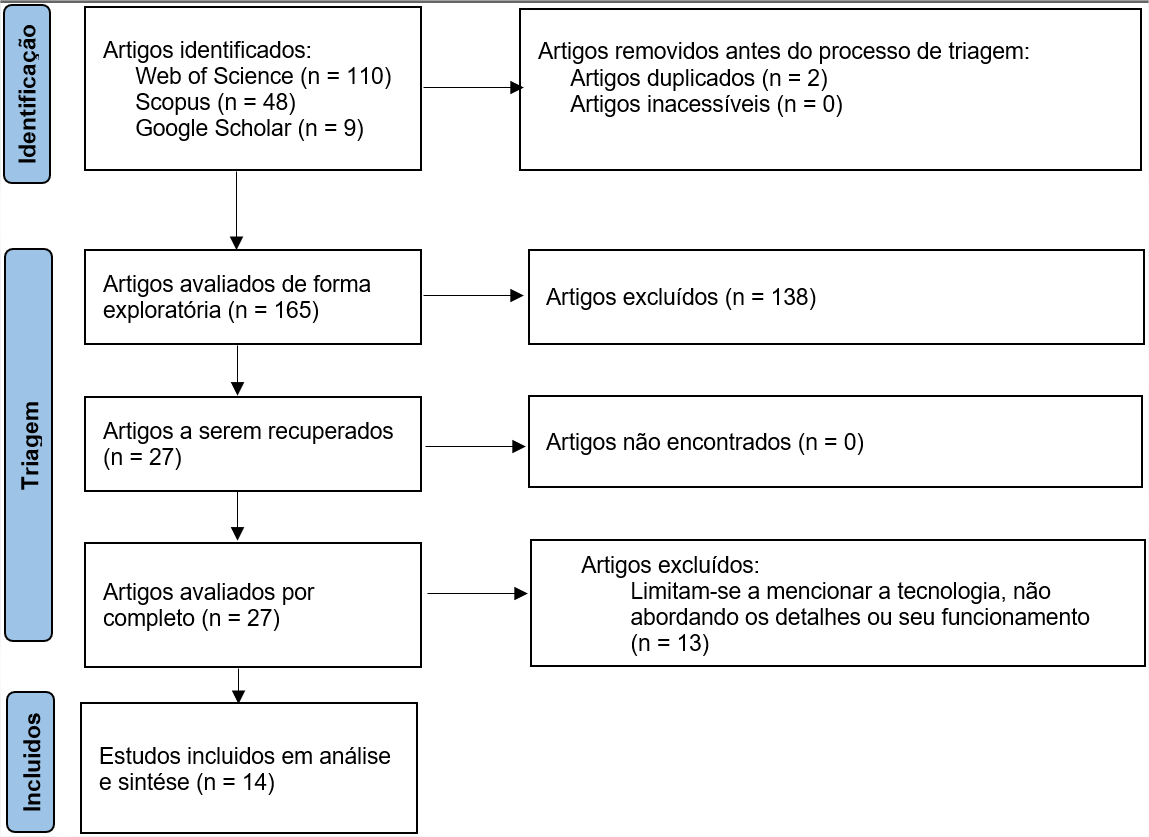
\includegraphics[width=0.8\textwidth]{imagens/Flux_revisao_sistematica_PRISMA.png} 
           \caption{Fluxograma da revisão sistemática conforme o protocolo PRISMA}
           \label{fig:flux_sistematic_revision}
        \end{figure}



%\subsection{Identificação}
%\label{subsec_identificacao}

    A primeira fase visa identificar os artigos na literatura. Para tal, é necessário definir uma base de dados, bem como a estratégia de busca. No presente trabalho, foram selecionadas as bases \textit{Web of Science, Scopus} e \textit{Google Scholar}.

    Em sequência, foi realizado o refinamento da \textit{string} de busca. Esta foi escolhida mediante testes nas bases e avaliações dos resultados obtidos. A \textit{string} final é composta pela junção das seguintes palavras-chave:

    \begin{itemize}
        \item String de busca em inglês:
        \begin{itemize}
            \item \textit{(Baggage OR Luggage OR Backpack OR Airport) AND}
            \item \textit{(Volume OR Size OR Dimension) AND}
            \item \textit{(point cloud OR Points OR Convex Hull OR Volume Detection OR Kinect OR Reconstruction OR “Object measurement”)}
        \end{itemize}
         \item String de busca em português:
        \begin{itemize}
            \item \textit{(Bagagem OU Mochila OU Bolsa OU Aeroporto) E}
            \item \textit{(Volume OU Tamanho OU Dimenção) E}
            \item \textit{(Nuvem de pontos OU Pontos OU Fecho Convexo OU Detecção de Volume OU Kinect OU Reconstrução OU “Medida de Objetos”)}
        \end{itemize}
    \end{itemize}
    
    A \textit{string} direciona o alcance da revisão a trabalhos que lidam com bagagens, contudo, o uso do operador “ou” permite a ocorrência de artigos aplicados em outros contextos que exploram medida de dimensões. Sendo assim, foi possível identificar 167 trabalhos. Note que, não foi adotado um limite de tempo para a busca. Os trabalhos retornados nessa etapa avançaram para a triagem.


%\subsection{Triagem}
%\label{subsec_triagem}

    A etapa inicial da triagem consistiu em uma leitura exploratória dos trabalhos para compreender se os mesmos são coerentes com a temática almejada. Nesta etapa, os artigos foram selecionados pela leitura do título, abstract e palavras-chave. Para realizar esse filtro, foram definidos os seguintes critérios de exclusão:

    \begin{enumerate}
        \item Descartar trabalhos que se limitam a detectar a presença da bagagem, mas não aborda o aspecto de sua dimensão ou volume;
        \item Descartar trabalhos que se limitam a detectar a presença de uma bagagem em situações isoladas, como em situações de segurança;
    \end{enumerate}

    Com base nos critérios definidos, foi possível remover 138 dos 167 trabalhos. A próxima etapa consistiu em recuperar os 27 trabalhos selecionados. Todos os trabalhos foram recuperados com sucesso, isto é, não houve problemas de acesso a nenhum deles. 

    Ainda no processo de triagem, realizou-se a leitura por completo dos trabalhos recuperados. Além dos critérios mencionados, descartaram-se trabalhos que apenas mencionam a detecção de dimensões, porém não entram em detalhes sobre os métodos ou tecnologias envolvidas. No final, foram incluídos 14 trabalhos. As próximas seções discorrem sobre os conceitos teóricos básicos e as informações obtidas por meio dos trabalhos selecionados.

\section{Fundamentação teórica}
\label{sec_Fundamentacao_teorica}

    A presente seção realiza uma breve revisão quanto aos conceitos que sustentam a teoria dessa pesquisa. Desse modo, serão discutidas as recomendações de dimensões para bagagens no Brasil, as ferramentas que podem ser utilizadas para extração das \textit{point clouds} e os métodos comumente utilizados para processá-las.

\subsection{Recomendações quanto às dimensões de bagagens}
\label{subsec_processo Processo de embarque}
    
    Para contextualizar o domínio de atuação desta pesquisa, é interessante considerar às recomendações quanto as dimensões das bagagens, especialmente na fase do check-in. É importante assinalar que o levantamento foi baseado na resolução nº 400 da agência Nacional de Aviação Civil \cite{anac_2022_resoluo}, mas podem ser customizadas pelas companhias aéreas. Por esse motivo, também foram consideradas empresas brasileiras, tal como \citeonline{azul_2022_bagagem} e a \citeonline{gol_2022_bagagem}.
    
	Prosseguindo, no check-in são apresentados os documentos necessários para embarque no voo, assim como, validação da bagagem de mão/porão. Por recomendação das companhias, isso deve ser feito com no mínimo 70 minutos de antecedência. Ao chegar no aeroporto, o passageiro terá que esperar pelo atendimento na fila de check-in, salvo se foi um processo remoto. Ainda nessa etapa também são despachadas as bagagens de porão e autorizadas as bagagens de mão, ambas mediante validação das medidas \cite{denis_2021_bagagem, daniel_2021_como}.
	
    O processo discutido revela a importância do tempo que o fluxo requer. Isso indica que os equipamentos utilizados para essa etapa devem ter o mais baixo consumo de tempo possível, dado que, alguns minutos já poderiam fazer o passageiro perder o voo. Quanto às bagagens, essas podem ser classificadas em três categorias \cite{azul_2022_bagagem}:
    
    \begin{itemize}
        \item \textbf{Bagagens de mão:} são levadas para a cabine da aeronave pelo próprio passageiro. Cada passageiro pode levar até 1 unidade sem taxa. Segundo a ANAC, os limites padrões para bagagens de mão são os seguintes: Altura: 55 cm; Largura: 25 cm; Profundidade: 35 cm e Peso máximo: 10 kg;
        \item \textbf{Bagagens de despacho:} devem ser entregues aos funcionários do aeroporto no balcão de check-in, ou para funcionários do despacho, a qual será enviada para o porão da aeronave. Cada passageiro pode levar até 1 unidade sem taxa. Segundo a ANAC, os limites padrões para bagagens de porão são os seguintes: Altura: 55 cm; largura: 80 cm; profundidade: 28 cm e Peso máximo: 23 kg.
        \item \textbf{Bagagens especiais}: São consideradas bagagens especiais aquelas que tem formato ou condição de manuseio diferentes do padrão (ex. malas de instrumentos, malas de itens de esporte), ou que estejam categorizadas como itens extras que não são contabilizados nas medidas (ex. tablet, notebook). Essa categoria é geralmente validada separadamente das demais malas. No caso, a Presente pesquisa não irá abordar em detalhes a medida desse tipo de mala.
    \end{itemize}
    
    É importante ter atenção às regras para dimensões e peso de bagagens estabelecidos pela companhia aérea contratada. Caso as malas excedam os limites, o passageiro terá que pagar uma taxa, caso contrário, poderá ser impedido de embarcar e orientado a realizar novamente o check-in. 


\subsection{Visão computacional e reconstrução de objetos 3D}
\label{subsec_Visão computacional e reconstrução de objetos 3D}

    Segundo \citeonline{zheng_2018_smart} e \citeonline{neethu_2015_role}, visão computacional é o processo de aquisição e análise de cenas reais (como vídeo e imagens) para tomada de decisões. O processamento das cenas, se dá por meio da aplicação de algoritmos de processamento digital de imagens, usados para extrair características e/ou tratar imagens. Por sua vez, tais características podem ser dados de entrada para modelos matemáticos, como, por exemplo, redes neurais. Ainda, segundo \citeonline{bhowmik_2018_embedded}, esses sistemas seguem um fluxo padrão de etapas, primeiro com uso de sensores para captura dos dados, posteriormente processamento, extração das características e, por fim, classificação.

    Quanto à reconstrução de objetos 3D, detalha-se que este é um ramo de estudo da visão computacional que visa reproduzir objetos do mundo físico no mundo digital, tendo, por sua vez, outros propósitos além da detecção das dimensões, tais como representar superfície e textura \cite{warnett_2016_towards, chen_2013_research}. Desse modo, existem duas vertentes, a reconstrução visual e a reconstrução ao nível de pontos. A presente pesquisa foca na segunda vertente, dado que a reconstrução é feita com intuito de obter-se as dimensões das bagagens, não sendo necessário realizar a reconstrução da superfície visual dos dados, conforme feito em trabalhos que focam em modelagem 3D. 



\subsection{Metrologia de termos utilizados nesse trabalho}
\label{subsec_Metrologia de termos utilizados nesse trabalho}
    
    A metrologia se dedica à pesquisa e à padronização dos procedimentos e terminologias relacionados a pesos e medidas. Neste trabalho, é importante ressaltar a definição adotada para algumas palavras frequentemente utilizadas ao descrever os resultados de testes. Essas palavras incluem "precisão," "acurácia" e "exatidão". Para tanto, foi utilizado como base o vocabulário internacional de metrologia presente em \cite{gov_2022_documentos} dentre outras fontes a serem citadas ao longo do texto.

    Prosseguindo, o termo \textit{precisão} refere-se ao grau de varição dos valores obtidos em um conjunto de medição, isso é, se o erro-padrão entre as medidas tem resultados próximos. Já a \textit{acurácia}, na presente pesquisa, se refere a proximidade do resultado medido ao valor tido como verdadeiro, significado semelhante ao de \textit{exatidão}, que também se refere ao grau de concordância entre um valor medido e um valor verdadeiro. Os autores do presente trabalho optaram pelo uso do termo \textit{exatidão}, uma vez que é definido em \citeonline{gov_2022_documentos}. Cabe destacar que, esses termos são qualitativos, por tanto, são necessários cálculos como erro absoluto médio (MAE) ou erro padrão para mensurar os valores \cite{gov_2022_documentos, zrhans_2018_acurcia}. 
    


\subsection{Ferramentas para amostragem de point clouds}
\label{sec_ferramentas para amostragem de point clouds}

    Com base nos resultados da revisão sistemática, observou-se uma multiplicidade de tecnologias que podem ser utilizadas para captura das dimensões de bagagens. O mesmo raciocínio se aplica aos algoritmos para tratamento dos dados, seja na remoção de ruídos, seja na junção dos pontos a serem processados. 

    Dentro do conjunto de tecnologias de captura, destaca-se o uso dos \textit{scanners a laser}, \textit{fixos e móveis}, \textit{câmeras binoculares} e \textit{sensores de profundidade} (ex. \textit{Microsoft Kinect}, \textit{Intel RealSense}).  A Figura \ref{fig:Disp_captura_ptClouds} lista os dispositivos citados.

        \begin{figure}[h]
           \centering
           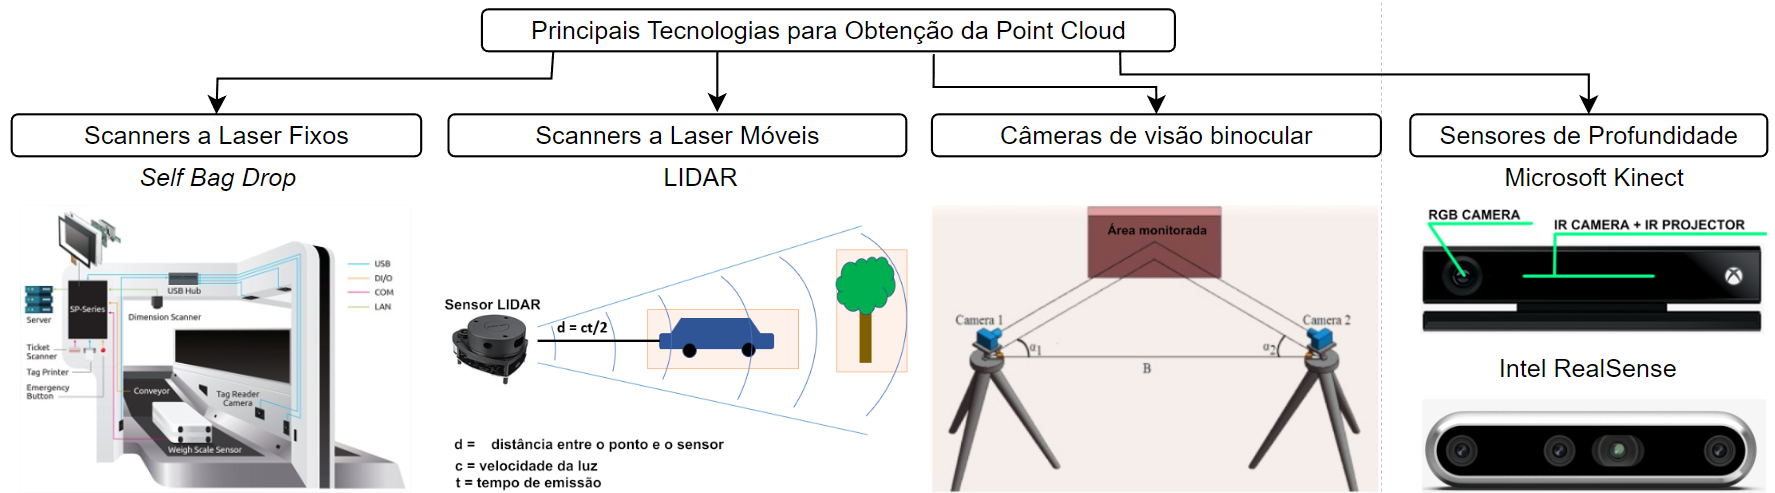
\includegraphics[width=1\textwidth]{imagens/Dispositivos_Para_captura_de_pt_Clouds.png} 
           \caption{Dispositivos para captura de \textit{point clouds}}
           \label{fig:Disp_captura_ptClouds}
        \end{figure}


\subsubsection{Sensores a laser fixos e móveis}
\label{subsec_Sensores a laser fixos e moveis}

    Os métodos que utilizam scanners a laser seguem uma de duas abordagens. A primeira é movimentar o laser ao longo do objeto, como em uma impressora. A segunda é mover o objeto ao longo de um eixo. Nesse caso, são definidas a velocidade do objeto e a taxa de amostragem do sensor, a partir disso, o laser coleta amostras de secções do objeto em forma de pontos no plano. Ao final do processo, todos os planos são combinados para formar uma point cloud em terceira dimensão \cite{gao_2018_minimum, hyypp_2020_accurate}. A Figura \ref{fig:Process_obterPtcloud_scanner} ilustra a segunda abordagem, usando uma esteira para mover o objeto.  

        \begin{figure}[h]
           \centering
           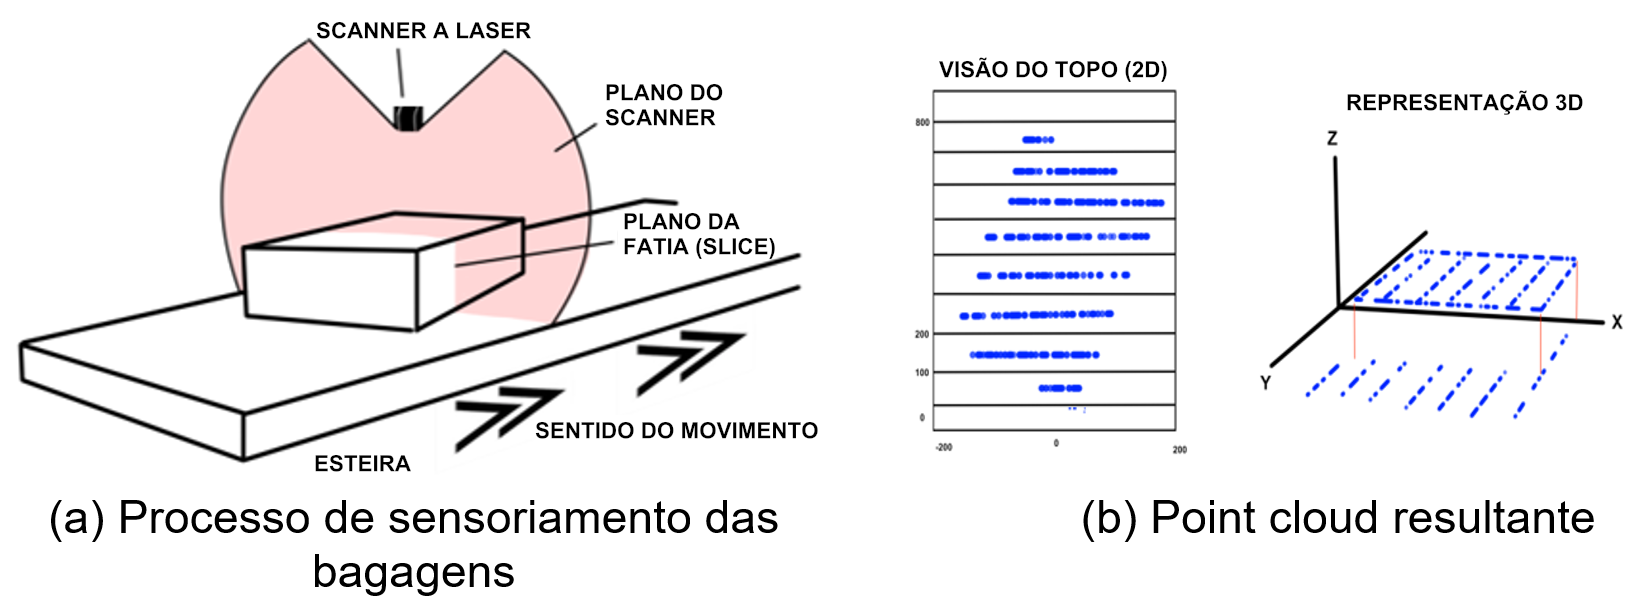
\includegraphics[width=1\textwidth]{imagens/Processo_Obtencao_pointCloud_com_scanner_laser.png} 
           \caption{Processo de obtenção de \textit{point clouds} com scanner a laser}
           \label{fig:Process_obterPtcloud_scanner}
        \end{figure}

    Quanto aos Scanners a laser fixos exemplificados nas Figuras \ref{fig:Disp_captura_ptClouds} e \ref{fig:sefl-bag-drop-URL_Disp}, estes, dentro do tema abordado, são aplicados em serviços de autoatendimento (self bag drop). Tais equipamentos são compostos por uma esteira, um ambiente interno com lasers e uma central de processamento \cite{qingji_2018_method}. O cliente coloca sua bagagem na esteira e o scanner, pelo uso dos sensores, retorna os valores de dimensões e/ou informações quanto a segurança e peso da bagagem \cite{gao_2018_minimum}. Esses equipamentos são os mais utilizados no mercado, porém, eles têm alto custo, são de uso específico e não apresentam tratamentos para casos excepcionais onde o cliente não posiciona as malas da forma padrão \cite{ren_2020_a, gao_2021_airline, qingji_2018_method}.

        \begin{figure}[h]
           \centering
           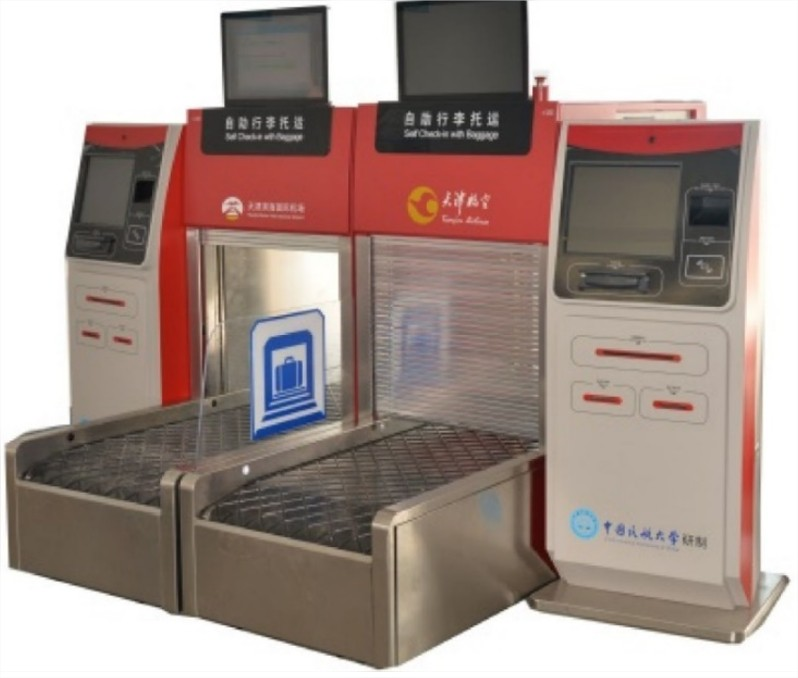
\includegraphics[width=0.5\textwidth]{imagens/self_bag_drop_10hz_40cm_s_URL_04LX.png} 
           \caption{Self bag drop de 10Hz e 40cm/s com Scanner URL-04LX \cite{gao_2018_minimum}}
           \label{fig:sefl-bag-drop-URL_Disp}
        \end{figure}

    
    Também cabe destacar dois pontos quanto ao posicionamento de self bag drops nas esteiras de atendimento, sendo eles \textit{one-step} (um-passo) e \textit{two-step} (dois-passos) \cite{neale_2017_automated}. O \textit{one-step} consiste da integração da esteira de medida de bagagem e de despacho, com isso o passageiro precisa posicionar a bagagem apenas uma vez, o que é mais eficiente e cômodo. O \textit{two-step} consiste em ter a esteira para medida de bagagens separada da de despacho. O passageiro precisa posicionar a bagagem primeiro no dispositivo para medida e depois transportá-la para a próxima etapa, é um processo com mais passos, porém, mais barato para a empresa. 
    
    Avançando na discussão, os scanners a laser móveis, exemplificado na Figura \ref{fig:Sensor LIDAR escaneando ambiente externo}, são aplicados no escaneamento de ambientes internos e externos \cite{zhang_2018_a}. A diferença ao modo fixo é que um operador ou veículo carrega o scanner, caminhando pelo cenário de modo a circundar a área para captura da \textit{point cloud} em 3D. 
    
        \begin{figure}[h]
           \centering
           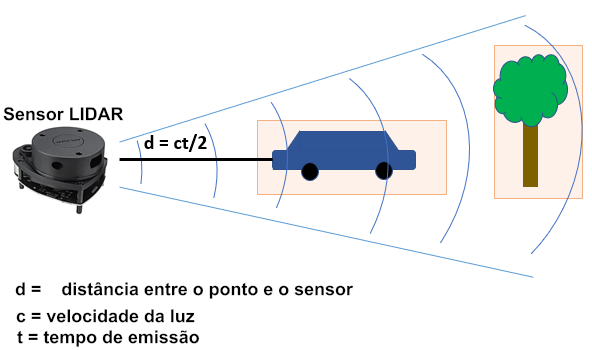
\includegraphics[width=0.5\textwidth]{imagens/Lidar_Sensor_metod.png} 
           \caption{Sensor LIDAR escaneando ambiente externo. Adaptado de \cite{mathworks_2022_introduction}}
           \label{fig:Sensor LIDAR escaneando ambiente externo}
        \end{figure}

    Ao longo do processo, o equipamento recebe as informações dos sensores e converte em \textit{point clouds}, que são tratadas pelo sistema interno de modo a eliminar valores atípicos (\textit{outliers}) \cite{xu_2021_lidar}. A partir disso, é possível reconstruir o ambiente explorado, seja com as funções do próprio equipamento, ou em softwares externos \cite{xu_2021_lidar, zhang_2018_a}. Para tanto, esses equipamentos geralmente utilizam sensores LiDAR (Detector de luz e espaço – \textit{Light Detection and Ranging}) que consegue obter informações de pontos a longas distâncias \cite{zhou_2019_extracting}.


\subsubsection{Câmeras comuns (visão binocular)}
\label{subsec_Cameras de visao binocular}

    Ainda quanto à geração da \textit{point cloud}, é importante mencionar os dispositivos que fazem uso da visão binocular. Essa técnica se assemelha à visão humana, envolvendo a captura de duas imagens do mesmo objeto por meio de câmeras, em ângulos ligeiramente diferentes. Com base nessas imagens, é possível criar uma representação tridimensional do objeto e determinar suas dimensões \cite{qingji_2018_method}. A principal desvantagem desse método, é que a posição da mala pode afetar significativamente o resultado, às vezes tornando esse método impraticável \cite{gao_2013_baggage}.

    Os sistemas que empregam essa técnica podem utilizar um dispositivo de visão binocular dedicado ou apenas coletar duas imagens em ângulos pré-definidos. A disposição das câmeras deve permitir a visualização da largura e altura do objeto. Em seguida, um algoritmo de correspondência de pontos é executado. Este, seleciona um ponto entre às duas imagens (foco) e analisa. Essa análise pode ser baseada no método de combinação em escalas de cinza ou na combinação de características. O algoritmo rastreia as duas imagens, pixel a pixel, mapeando os pontos dos índices (x, y) do R2 em pontos (x, y, z) no R3 espaço em x, y e z \cite{sun_2019_threedimensional, qingji_2018_method, li_2017_the}. A Figura \ref{fig:visao_binocular} mostra o modelo para captura de um ponto no espaço utilizando a técnica da visão binocular.

        \begin{figure}[h]
           \centering
           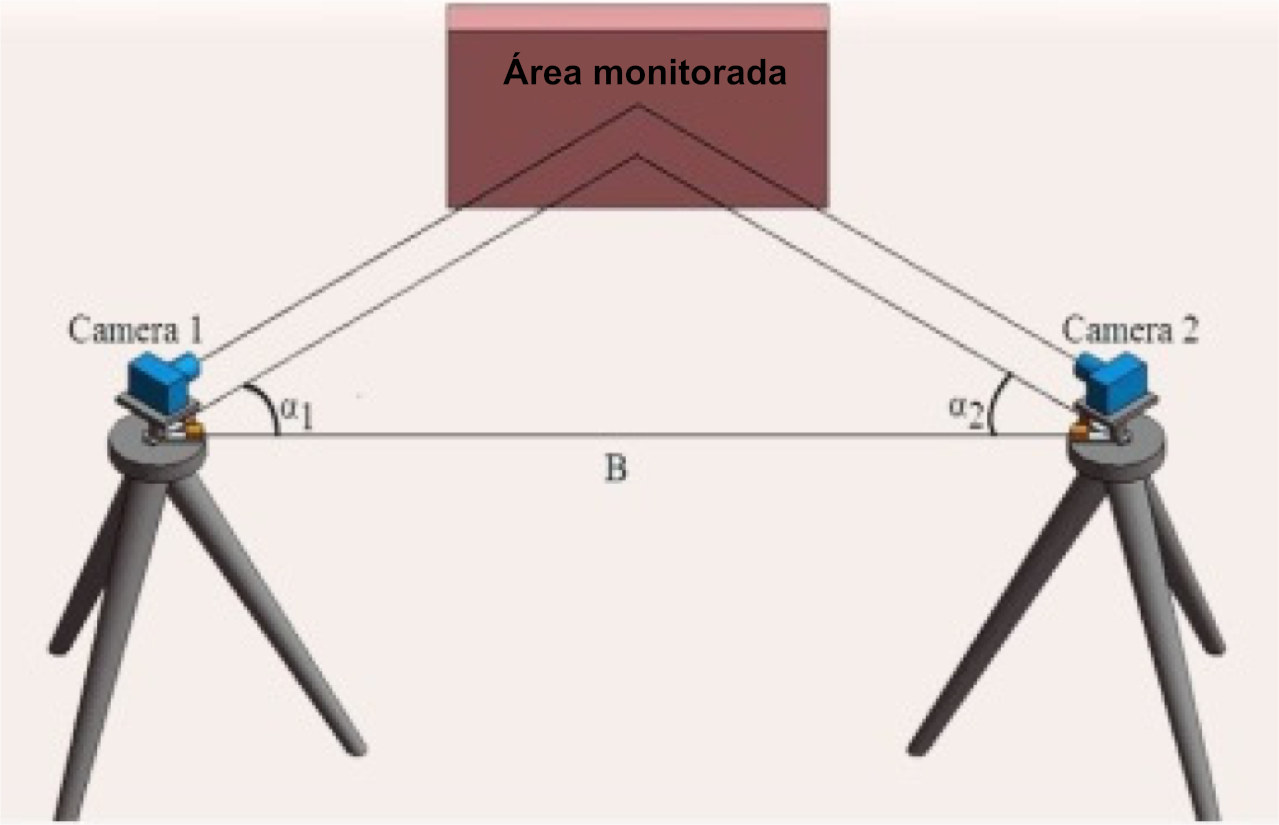
\includegraphics[width=0.45\textwidth]{imagens/capturaDeUmPontoComVisaoBinocular.png} 
           \caption{Captura de um ponto com visão binocular. Adaptado de \cite{hu_2020_accuracy}}
           \label{fig:visao_binocular}
        \end{figure}
    

\subsubsection{Sensores de profundidade}
\label{subsec_Sensores de profundidade}

    Como alternativa para as tecnologias mencionadas, pesquisadores exploram os sensores de profundidade, como o Kinect e o \textit{intel realsense} \cite{ruchay_2018_fusion}. O sensor kinect, inicialmente desenvolvido pela Microsoft para videogames \cite{chan_2018_an}, tem demonstrado sua utilidade e eficiência em pesquisas científicas, sendo capaz de gerar \textit{point clouds} com alta precisão e rapidez \cite{chen_2013_research}. Além disso, seu baixo custo, em torno de 200 dólares, o torna uma opção viável para a criação de sistemas de visão de baixo custo \cite{wan_2012_a}. A Figura \ref{fig:Kinectv2}, representa um Kinect versão 2 e seus requisitos de hardware.
    
        \begin{figure}[h]
           \centering
           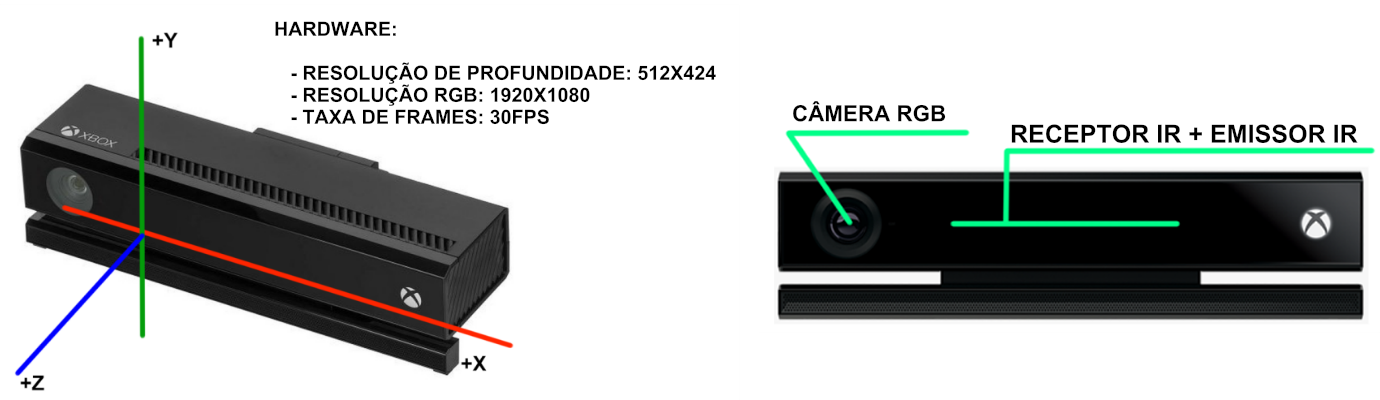
\includegraphics[width=1\textwidth]{imagens/KinectV2.png} 
           \caption{Kinect V2}
           \label{fig:Kinectv2}
        \end{figure}

    Quanto ao hardware, o Kinect é composto por três lentes. Duas dessas lentes funcionam como emissor e receptor de infravermelho, sendo responsáveis por capturar informações de profundidade da cena. A terceira lente é uma câmera RGB que opera a 30 quadros por segundo (fps), com resolução de 640x480 pixels na versão 1.0 e 1920x1080 pixels na versão 2.0. O Kinect 2.0 apresentou diversas melhorias, incluindo o aumento da resolução da câmera RGB e a correção de alguns problemas relacionados ao rastreamento de movimento \cite{chan_2018_an, ruchay_2018_fusion}.
    
    Com isso, os principais elementos que podem ser capturados via Kinect v2 são uma imagem RGB, uma imagem de profundidade e a \textit{point cloud}. A \textit{colorImage} (imagem RGB) pode ser utilizada para colorir a \textit{point cloud}, permitindo o estudo, por exemplo, de textura.  A \textit{depthImage} (imagem de profundidade) contém os dados de profundidade, largura e altura de cada ponto, dado que, devido ao alcance dos sensores IR, às dimensões são de 512 x 424.
        
    Quanto ao alcance de captura do Kinect, este tem o limite máximo de 8 m e mínimo de 0,4 m. No entanto, a distância que retorna medidas mais precisas tem o máximo de 3 m e o mínimo de 0,5 m, a precisão de medição se altera conforme a distância do objeto partindo de 1 mm a 10 cm \cite{guffanti_2020_the}. 
        
    Avançado na discussão, outra opção de sensor de profundidade é o\textit{intel realsense}, distribuído em vários modelos. Considerando a linha D400 no modelo D450, tem-se que a resolução da câmera de profundidade é de 1280 x 720 com até 90 fps, sendo o espaço de alcance de 0.6 m até 6 m e 2\% de precisão. Já a câmera RGB tem 1280 x 800 pixels de resolução com até 30 fps, equivalente ao do kinect v2 \cite{intel_2021_introducing}.

    A técnica de captura utilizada pelos sensores de profundidade envolve a emissão de um raio infravermelho que, ao entrar em contato com um objeto, é refletido de volta e capturado pelo receptor. O sistema interno recebe essa informação e constrói um ponto no espaço (x, y e z). Esse processo é repetido ao longo dos limites do campo de visão do dispositivo, resultando em uma matriz de profundidade (\textit{depth image}), com todos os pontos em unidades de metros (m). Ainda, é possível obter uma \textit{point cloud} colorida, gerada a partir do mapeamento dos pixels da imagem RGB (\textit{color image}) nos pontos da imagem de profundidade \cite{mathworks_2017_acquire, jiao_2017_a}. A Figura \ref{fig:ColetandopointCloudComSensorDeProfundidade} mostra um processo genérico para coleta de \textit{point cloud} de um objeto utilizando um sensor de profundidade.
    
        \begin{figure}[h]
           \centering
           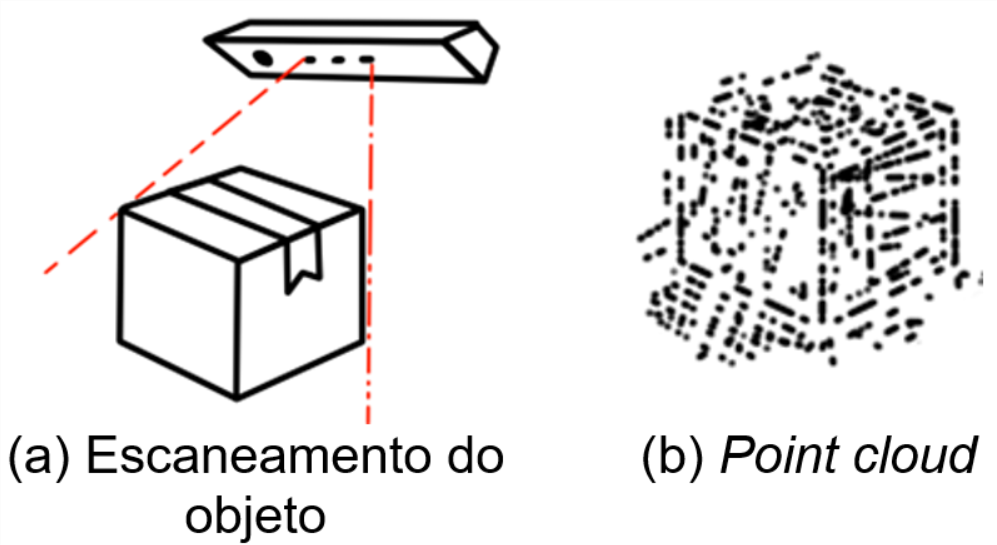
\includegraphics[width=0.6\textwidth]{imagens/processoDeObtencaoPointCloudSensorProfundidade.png} 
           \caption{Processo de obtenção da \textit{point cloud} usando um sensor de profundidade}
           \label{fig:ColetandopointCloudComSensorDeProfundidade}
        \end{figure}


\subsection{Comparação entre tecnologias para atividades operacionais em terminais aeroportuários}
\label{sec_Comparação entre tecnologias}

    Na presente seção será realizada uma comparação entre as soluções retornadas pela revisão e outras tecnologias. Para tanto, foi utilizada a metodologia proposta por \citeonline{ronzani_2019_explorao}, que estabelece uma abordagem para medição de desempenho entre tecnologias de monitoramento operacional em terminais aeroportuários. Nessa abordagem, cada elemento é avaliado com base em Indicadores de Performance Chave (KPI - \textit{Key Performance Indicators}), critérios que permitem avaliar as tecnologias de forma agrupada, independente de sua aplicação no aeroporto. Por meio desses critérios é possível avaliar fatores gerais e de automação proporcionada pelo equipamento. Os principais KPIs propostos pela pesquisa citada e aqui utilizados, são os seguintes:
    
    \begin{enumerate}
        \item Precisão: capacidade de capturar corretamente os dados de interesse;
        \item Automação: equipamentos que exigem operação pelo passageiro, estão mais suscetíveis a interferências no fluxo;
        \item Confiabilidade: quanto maior a participação de indivíduos, mais suscetível a erros ou falhas o sistema é. Os equipamentos eletrônicos operam com pouco ou nenhum efeito humano no controle, agilizando, também, a correção de erros;
        \item Segurança: se refere a segurança em se utilizar o equipamento, pode ser avaliada por meio de questionamentos tais como:  A tecnologia lê a bagagem? A tecnologia encontra as dimensões? É confiável  que o passageiro vai pegar a mala de volta após passar pelo equipamento? É seguro utilizar essa tecnologia?;
        \item Custo/tempo de implantação: se refere ao custo do equipamento e o tempo para integração da nova tecnologias nas dependências do aeroporto;
        \item Custo de operação e manutenção: se refere ao custo envolvido na utilização do equipamento, por exemplo, se ele é totalmente automatizado, então o custo é menor com funcionários. O custo de manutenção tem relação com os ajustes necessários e os gastos para manter o dispositivo funcional e com peças adequadas.
    \end{enumerate}

    A partir dos KPIs o método propõe a comparação entre as tecnologias por meio de uma tabela de multicritérios ponderados. São atribuídos pesos de 1 a 3, sendo 1 uma avaliação ruim, 2 uma avaliação regular e 3 uma avaliação boa. Com base nisso, foi gerada a Tabela \ref{tab:avaliao_relativa} que faz a comparação relativa entre as tecnologias levantadas na revisão sistemática e algumas fora do escopo desse trabalho, mas indicadas em \cite{ronzani_2019_explorao}. A Figura \ref{fig:graficos_comparacao_entre_tecnologias} expõe os dados de forma gráfica, comparando os resultados para cada KPI individualmente. 
    

\begin{table}[h!]
\centering
\resizebox{\textwidth}{!}{%
\begin{tabular}{llccccccc}
\hline
ID &
  Tecnologia &
  \multicolumn{1}{l}{Precisão} &
  \multicolumn{1}{l}{Automação} &
  \multicolumn{1}{l}{Confiabilidade} &
  \multicolumn{1}{l}{segurança} &
  \begin{tabular}[c]{@{}c@{}}Custo e\\ tempo de implantação\end{tabular} &
  \begin{tabular}[c]{@{}c@{}}Custo de operação e \\ manutenção\end{tabular} &
  \multicolumn{1}{l}{Média} \\ \hline
1 & Sensores de profundidade           & 2 & 3 & 2 & 3 & 3 & 3 & 2,67 \\
2 & Câmeras Comuns (Visão binocular) & 2 & 2 & 3 & 3 & 3 & 3 & 2,67 \\
3 & Scanner a laser fixo             & 3 & 3 & 3 & 3 & 1 & 1 & 2,33 \\
4 & Scanner a laser móvel            & 2 & 1 & 2 & 2 & 1 & 1 & 1,50 \\
5 & Leitor de QR Code                & 3 & 1 & 1 & 3 & 2 & 3 & 2,17 \\
6 & RFID                             & 3 & 2 & 2 & 3 & 2 & 3 & 2,50 \\
7 & Sensores Estereoscópicos 3D      & 2 & 3 & 2 & 3 & 1 & 2 & 2,17 \\
8 & Contador infravermelho           & 2 & 3 & 2 & 2 & 2 & 2 & 2,17 \\ \hline
\end{tabular}%
}
\caption{Avaliação relativa entre as soluções levantadas nessa pesquisa e demais  soluções tecnológicas}
\label{tab:avaliao_relativa}
\end{table}



        \begin{figure}[h]
           \centering
           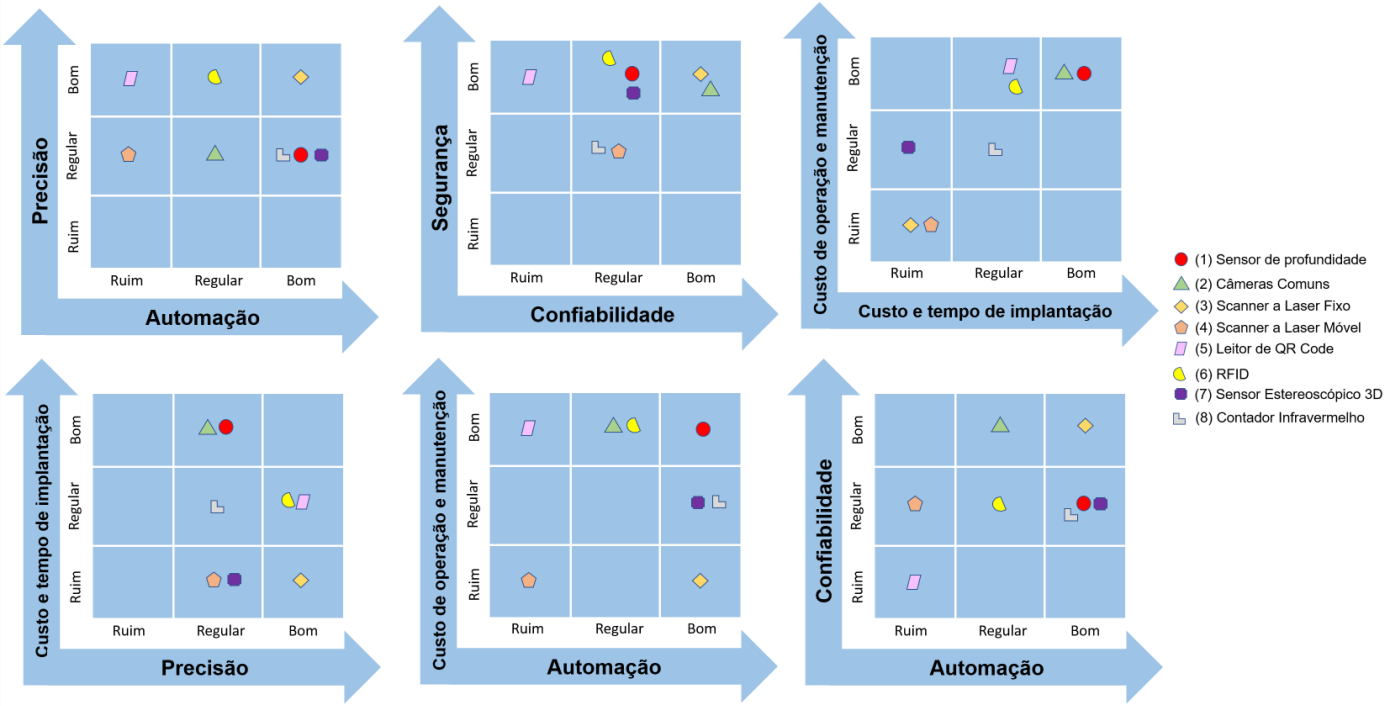
\includegraphics[width=1\textwidth]{imagens/graficos_comparacao_entre_tecnologias.png}
           \caption{Gráficos de comparação relativa entre as soluções levantadas e outras do mercado}
          \label{fig:graficos_comparacao_entre_tecnologias}
        \end{figure}


Pela observação dos dados expostos na Tabela \ref{tab:avaliao_relativa} e na figura \ref{fig:graficos_comparacao_entre_tecnologias} é possível realizar algumas pontuações. Quanto à precisão, tem-se que as tecnologias 3, 5 e 6 obtiveram avaliação boa, já as demais soluções ficaram regulares. As tecnologias 1, 2, 3 e 7 tiveram, em média, boa avaliação em automação, confiabilidade e segurança, isso porque elas têm pouca ou nenhuma necessidade de intervenção humana no processo e, consequentemente, retornam resultados mais confiáveis, promovendo a segurança das bagagens já que existe pouca manipulação humana e, por vezes, o passageiro consegue acompanhar visualmente o processo. Por fim, as tecnologias 1 e 2 receberam boa avaliação em custos e tempo envolvidos na implantação, operação e manutenção, isso por que esses equipamentos têm boa usabilidade e peças de baixo custo. 

Prosseguindo, a Tabela \ref{tab:avaliao_relativa} mostra que as tecnologias para medida de bagagens, no caso o  Scanner a laser fixo, câmeras comuns e sensores de profundidade, ficaram bem próximos. Nesse cenário, a empresa tem que considerar o custo benefício da tecnologia e sua aplicação no aeroporto para decidir qual equipamento utilizar.

Nessa situação, outros fatores que podem ser considerados na aquisição de uma solução automatizada em detrimento de uma manual são a disponibilidade dos dados, detalhamento de padrões e subsídio a gestão comercial e operacional. Quanto à disponibilidade dos dados, sistemas manuais exigem mais tempo, já os automáticos fazem isso em segundos. Quanto ao detalhamento de padrões, os fatores humanos podem influenciar os resultados de cada aferição, em contrapartida, os sistemas automáticos reproduzem padrões no método e nos resultados. Por fim, quanto ao subsídio da gestão comercial e operacional, os sistemas automatizados podem coletar dados mais completos e precisos, possibilitando que gestores produzam análises mais aprofundadas.




\subsection{Métodos e algoritmos comumente utilizados}
\label{sec_Metodos e algoritmos comumente utilizados}

    De modo geral, as tecnologias utilizadas pela indústria aplicam técnicas de visão computacional e reconstrução de objetos 3D para obter a dimensão de objetos. Esse processo é feito tipicamente a partir de uma \textit{\textit{point cloud}} (nuvem de pontos), coletada via sensor. Esta, é um conjunto de informações representadas por pontos no plano ou no espaço. No presente contexto corresponde a pontos no espaço extraídos da superfície de uma bagagem \cite{chen_2013_research}.
    
    Posteriormente, os pontos podem ser delimitados em um polígono tridimensional para cálculo de dimensões. A literatura indica que é comumente empregado o algoritmo de convex hull (fecho convexo) para obtenção do menor polígono que envolve os pontos do objeto capturado \cite{neethu_2015_role, gao_2018_minimum, ding_2018_a}.

    Antes da análise da \textit{point cloud}, são usualmente executados algoritmos de pré-processamento. Em tal etapa podem ser aplicadas técnicas tais como \textit{subamostragem}, \textit{clusterização} e os filtros de \textit{média, bilateral e Gaussiano}. A subamostragem reduz a densidade de pontos, diminuindo o gasto computacional \cite{ruchay_2018_fusion}. Já a clusterização, remove \textit{outliers} que podem atrapalhar o processo de reconstrução, por exemplo, um ponto extremo pode mudar significativamente o polígono que delimita o objeto 3D. Métodos dessa categoria	  possibilitam, também, agrupar informações semelhantes, o que pode acelerar o processamento das etapas posteriores. DBSCAN (Seção \ref{subsec_Metodos para Clusterização}) e k-means são exemplos de algoritmos nesse escopo \cite{limwattanapibool_2017_determination}. 

    Da mesma forma podem ser aplicados filtros para normalizar pontos e ressaltar saliências, como bordas das bagagens \cite{ruchay_2018_fusion}.  Os Filtros bilateral e Gaussiano, reduzem erros de granulação nos cantos e de componentes de alta frequência \cite{shin_2014_implementation, wan_2012_a}. As próximas subseções entram em detalhes quanto aos métodos aplicados na presente pesquisa.

\subsubsection{Métodos para obtenção de dimensões}
\label{subsec_Metodos para obtenção de dimensões}

    Para manipulação da \textit{point cloud}, comumente se utilizam os algoritmos de fecho convexo (convex hull) \cite{ding_2018_a}. Dado um conjunto de pontos A, estes algoritmos operam de modo a encontrar os pontos da extremidade gerando um subconjunto B, que, por sua vez, representa o menor polígono que reveste todos os pontos da \textit{point cloud} \cite{zhao_2018_3d}. Tal polígono, ou polígonos, podem ser utilizados para reproduzir a superfície dos objetos ou coletar informações de dimensões. A Figura \ref{fig:AplicacaoConvexHull2D3D} ilustra a aplicação do algoritmo citado em 2D e 3D.

        \begin{figure}[h]
           \centering
           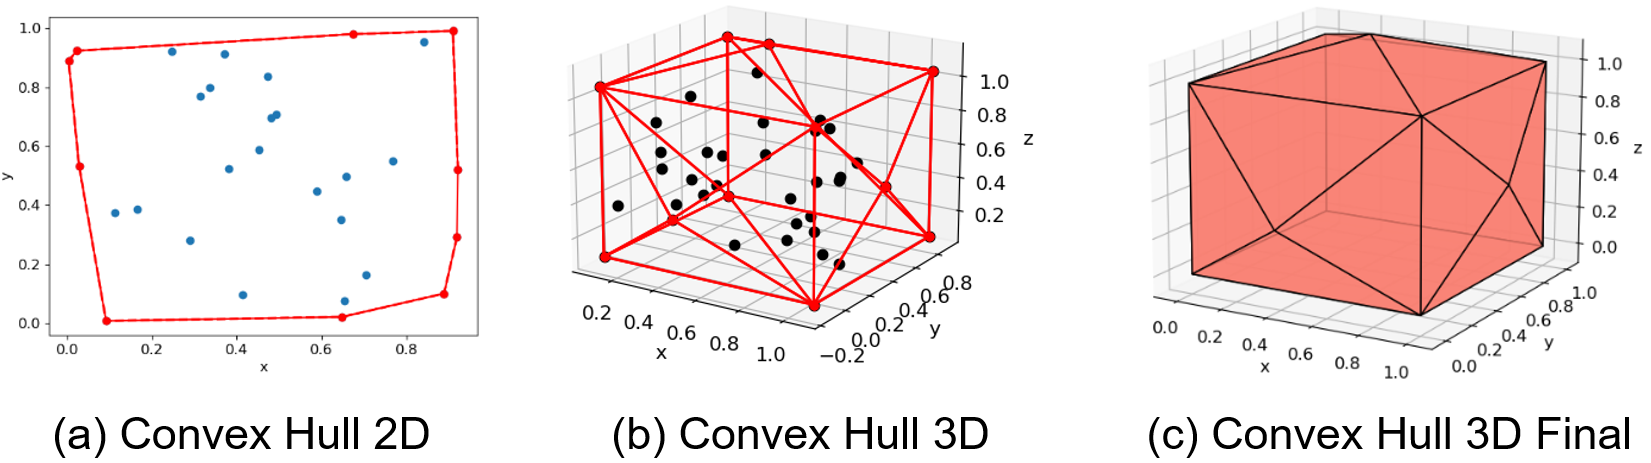
\includegraphics[width=0.9\textwidth]{imagens/aplicacaoConvexHullEmPtCloud2D3D.png} 
           \caption{Aplicação convex hull em 2D e 3D}
           \label{fig:AplicacaoConvexHull2D3D}
        \end{figure}


    No plano (2D), o convex hull é o menor polígono que contém um conjunto de pontos $P$. Já no espaço (3D), o convex hull  é a menor figura tridimensional que reveste o conjunto de pontos $P$. A Figura \ref{fig:AplicacaoConvexHull2D3D} ilustra o resultado para ambas as situações citadas. Outro detalhe, é que o convex hull 3D representa todas as combinações ou concatenação de conjuntos $P_x$ de pontos no plano 2D extraídos do conjunto $P_y$ de pontos no espaço 3D. Isso implica que ele é construído por meio da repetição do convex hull 2D em todo o conjunto de $P_x$ pontos disponíveis, sendo que o conjunto resultante $P_y$, consequentemente, contém o conjunto $P_x$ \cite{zhao_2018_3d,laurini_2017_geographic}. 
	
   
%\subsubsection{Métodos de caixas mínimas limitantes}
%\label{subsec_Metodos de caixas Mínimas limitantes}


    Avançando no tópico, outra opção para obtenção de dimensões são os algoritmos de caixas mínimas limitantes (\textit{minimun bounding box} -- MBB). Assim como o convex hull, que simplifica a forma original do objeto, esses algoritmos consideram qualquer forma como uma caixa. Nesse contexto, o objetivo é encontrar a figura retangular de menor área que envolve um conjunto $P$ de pontos. Para tanto, são rastreados os limites da \textit{point cloud} de modo a identificar os maiores e menores valores de x, y e z \cite{siwei_2021_review}. Essa abordagem é interessante, pois a partir desse polígono é possível extrair informações de largura, comprimento e profundidade, com boa exatidão e sem a necessidade de tratar todos os pontos do conjunto \cite{actorsfit_2021_pcl_pcaminimum}. 
    
    Na literatura são identificadas muitas variações do MBB, sendo as principais o de caixas mínimas alinhadas com os eixos (\textit{Aligned Axis Bounding Box} -- AABB) e caixas mínimas orientadas (\textit{Oriented Minimum Bounding Box} -- OMBB). A Figura \ref{fig:MBBsilustracoes} ilustra os métodos citados assim como a aplicação em três dimensões.

        \begin{figure}[h]
           \centering
           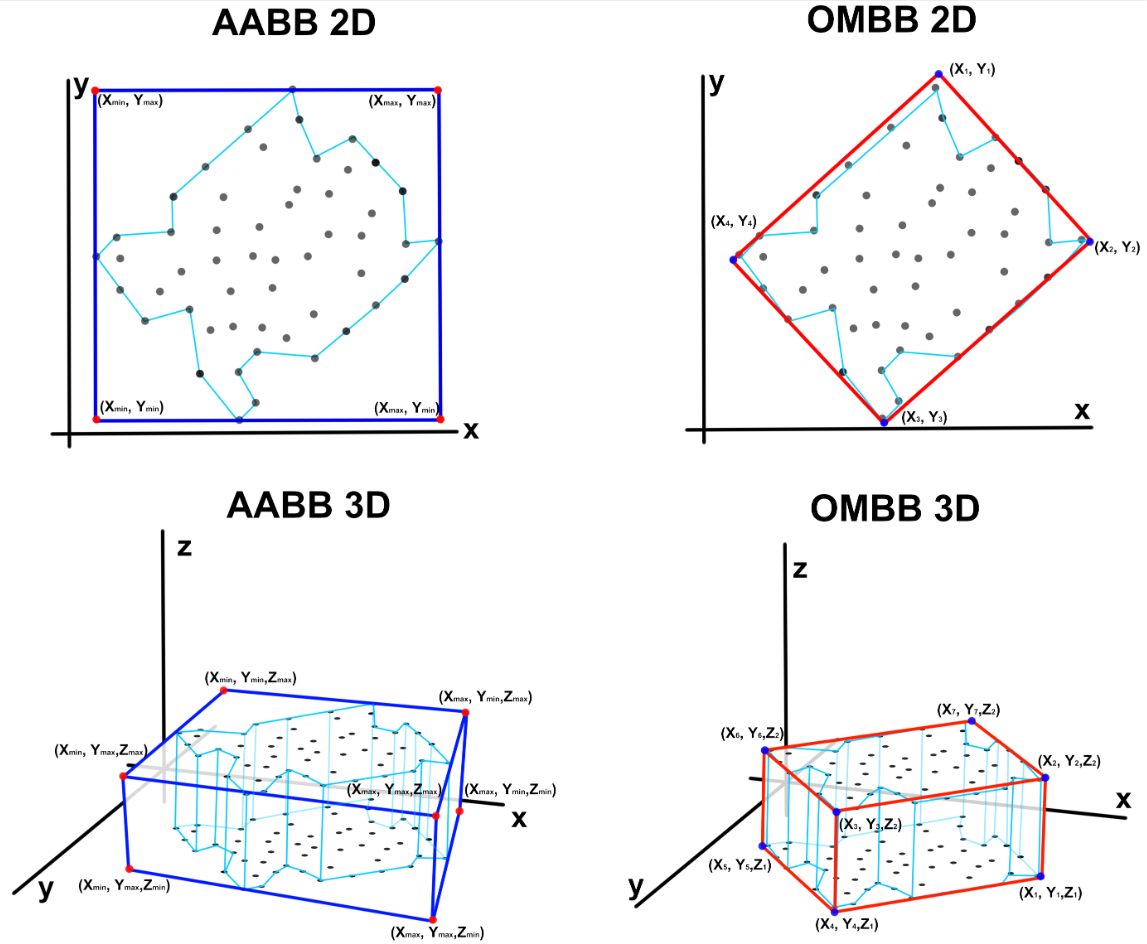
\includegraphics[width=0.8\textwidth]{imagens/MBBs ilustracoes.png} 
           \caption{AABB e OMBB 2D e 3D, convex hull em azul-claro. Adaptado de \cite{david_2014_computing}}
           \label{fig:MBBsilustracoes}
        \end{figure}
    
    Segundo \citeonline{siwei_2021_review} o AABB é o método mais simples dessa categoria e promove um processamento rápido. Neste caso, dada uma \textit{point cloud}, são computados os pontos localizados nas extremidades máximas e mínimas considerando apenas os eixos do plano, sem avaliar se o objeto está rotacionado. Tais pontos representam os vértices de um retângulo que engloba a \textit{point cloud}.  Os módulos dos vetores traçados entre os pontos correspondem aos escalares das dimensões.

    Já o OMBB é definido como o menor retângulo que engloba os pontos, podendo este estar em posição arbitrária em relação aos eixos. Esse método é mais complexo que o AABB, no entanto, é mais preciso, uma vez que consegue obter a menor medida considerando a orientação dos pontos \cite{siwei_2021_review}. Para medida de bagagens, esse método pode aumentar a exatidão do sistema em casos que a mala seja posicionada de outras formas que não a padrão (ex. rotacionada na diagonal). Uma das abordagens para obter o OMBB pode ser resumida nos passos ilustrados na  Figura \ref{fig:fluxogramaOMBB} \cite{david_2014_computing}.

        \begin{figure}[h]
           \centering
           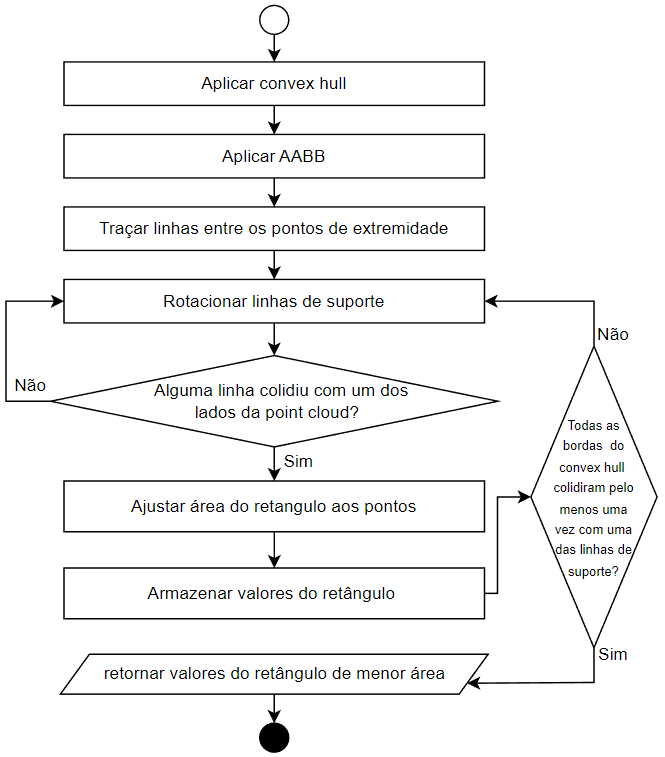
\includegraphics[width=0.6\textwidth]{imagens/fluxogramaOMBB.png} 
           \caption{Fluxograma OMBB. Adaptado de \cite{david_2014_computing}}
           \label{fig:fluxogramaOMBB}
        \end{figure}

    Os métodos supracitados também podem ser aplicados em 3D. Uma abordagem para obter esse resultado é dividir o cenário 3D em vários casos de pontos em 2D. Desse modo é possível aplicar o AABB ou o OMBB nos N planos resultantes da divisão. Uma forma de dividir o cenário é processar uma face do cuboide por vez aplicando os processos nos planos (xy, xz, yz), ou segmentar os pontos em N planos em níveis diferentes do eixo Z \cite{siwei_2021_review, mousavian_2017_3d}.
   
   
    
\subsubsection{Métodos para Clusterização}
\label{subsec_Metodos para Clusterização}

    O DBSCAN é um método de agrupamento de pontos em clusters, sendo o principal identificado na literatura no presente escopo. O algoritmo busca encontrar áreas de grande densidade de pontos que estão separadas por áreas com baixa densidade para as agrupar, formando assim, clusters (conjuntos) \cite{schubert_2017_dbscan, harman_2020_dbscan}. É possível utilizar tal método para segmentação de imagens ou de pontos, filtragem, classificação de objetos e remoção de ruídos. Para tanto, o algoritmo rastreia os pontos classificando-os em uma de três opções, as quais são: 
    
    \begin{itemize}
        \item \textbf{Pontos de núcleo (Core points):} são pontos que tem uma vizinhança grande o suficiente para formar um cluster, isso é dado pelo valor de “pontos mínimos”;
        \item \textbf{Pontos de borda (Border Points):} são pontos que não têm os pontos mínimos para formar um cluster, porém fazem parte do cluster de algum ponto de núcleo;
        \item \textbf{Pontos de ruído:} são pontos que não têm uma vizinhança grande o suficiente para formar um cluster e também não fazem parte de algum outro cluster. 
    \end{itemize}
    
    Para realização da classificação, o DBSCAN trabalha com 3 parâmetros, mostrados na Figura \ref{fig:classificacaoPontosDbScan}, sendo eles os seguintes:
    
    \begin{itemize}
        \item \textbf{$\epsilon$ :} se refere ao tamanho do raio de um cluster. Ou seja, os clusters podem ser representados visualmente como um círculo de raio $\epsilon$. Pelo cálculo da distância, se um ponto $P_i$  de  $P$ estiver no raio $\epsilon$ de um conjunto $A$, ele faz parte deste conjunto; 
        \item \textbf{MinPts:} é a quantidade mínima de pontos necessários dentro do alcance de $\epsilon$ para ser considerado um cluster;
        \item \textbf{Vizinhança:} a vizinhança de um ponto $P_i$ é dada pela distância limitada pelo valor de $\epsilon$.
    \end{itemize}
    
        \begin{figure}[h]
           \centering
           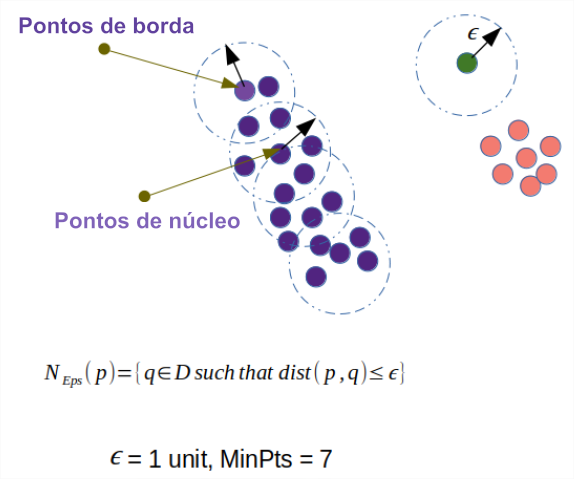
\includegraphics[width=0.5\textwidth]{imagens/classificacaoPontosDbScan.png} 
           \caption{Classificação dos pontos e definição dos clusters em uma \textit{point cloud} (DBSCAN) \cite{harman_2020_dbscan}}
           \label{fig:classificacaoPontosDbScan}
        \end{figure}
    
    
    A partir da teoria descrita, é possível perceber que o DBSCAN pode ser aplicado para diversos fins. Ele é capaz de separar vários conjuntos de pontos em clusters, independentemente do formato da \textit{point cloud} e mesmo que esses conjuntos estejam distantes uns dos outros. Além disso, o DBSCAN pode ser utilizado como um filtro para remover \textit{outliers}, identificando não apenas pontos de borda, mas também pontos que estão isolados do cluster principal.
    

\section{Trabalhos relacionados}
\label{sec_Trabalhos relacionados}

    Assim como indicado na Figura \ref{fig:flux_sistematic_revision}, foram analisadas as abordagens dos trabalhos selecionados. A Tabela \ref{tab:revisaoSistematica} sintetiza as principais características de tais trabalhos conforme o tipo de objeto. Observou-se que todos os artigos analisados operam utilizando \textit{point clouds}. O que os difere é como os mesmos a obtêm, bem como quais técnicas são empregadas para extrair as medidas dos objetos.





\subsection{Abordagens principais e complementares}
\label{subsec_Abordagens principais e complementares}

    Tomando como referência a Tabela \ref{tab:revisaoSistematica}, os três primeiros trabalhos realizaram a detecção de dimensões de bagagens em aeroportos. Os demais, atuaram em outros contextos, os quais serão analisados segundo a aplicabilidade no problema em questão. A seguir são discutidas de forma pontual as informações obtidas.



\begin{table}[h!]
\centering
\resizebox{\textwidth}{!}{%
\begin{tabular}{@{}llllll@{}}
\toprule
Trabalho & Tecnologia base & Tipo de Objeto & Mult. objetos & Complexidade do objeto & Posição do Objeto \\ \midrule
\citeonline{gao_2018_minimum} & Scanner a laser & Bagagens & Não & Uniforme & Limitado \\
\citeonline{qingji_2018_method} & \begin{tabular}[c]{@{}l@{}}Câmera estereoscópica \\ binocular HD e projetor\end{tabular} & Bagagens & Não & Uniforme & Limitado \\
\citeonline{gao_2013_baggage} & \begin{tabular}[c]{@{}l@{}}Duas câmeras com as \\ mesmas especificações\end{tabular} & Bagagens & Não & \begin{tabular}[c]{@{}l@{}}Deformações \\ leves\end{tabular} & Limitado \\
\citeonline{ozbay_2013_3d} & 1 Microsoft Kinect & Mobília, copos e cadeiras & Não & Uniformes e Curvos & Qualquer posição \\
\citeonline{chen_2013_research} & 1 Microsoft Kinect & Caixas e obj. complexos & Não & Deformações grandes & Limitado \\
\citeonline{ruchay_2018_fusion} & 4 Microsoft Kinect & Genérico, teste com cadeira & Não & Uniformes e Curvos & Qualquer posição \\
\citeonline{wan_2012_a} & 1 Microsoft Kinect & Genérico, teste com pessoas & Não & Deformações grandes & Limitado \\
\citeonline{shin_2014_implementation} & 2 Microsoft Kinect & \begin{tabular}[c]{@{}l@{}}Genérico, teste com pessoas\\  e móveis\end{tabular} & Não & Deformações grandes & Qualquer posição \\
\citeonline{sun_2019_threedimensional} & 1 Microsoft Kinect v2 & Genérico, teste com árvore & Não & \begin{tabular}[c]{@{}l@{}}Deformações grandes \\ com Lacunas\end{tabular} & Limitado \\
\citeonline{chan_2018_an} & 1 Microsoft Kinect v2 & Alimentos & Não & Curvos & Limitado \\
\citeonline{ryu_2020_algorithm} & Scanner a laser & \begin{tabular}[c]{@{}l@{}}Ambiente interno \\ (ex. sala e paredes)\end{tabular} & Sim & Uniforme & Qualquer posição \\
\citeonline{hyypp_2020_comparison} & Sensor a laser móvel & Obj. Complexos (árvores) & Sim & Curvos e Lacunas & Qualquer posição \\
\citeonline{warnett_2016_towards} & \begin{tabular}[c]{@{}l@{}}Raio-X CT e Scanner \\ a Laser\end{tabular} & Produto em metal & Não & Uniformes e Curvos & Qualquer posição \\
\citeonline{zhou_2019_extracting} & Scanner a Laser Móvel & Obj. Complexos (árvores) & Sim & Deformações grandes & Qualquer posição \\ \bottomrule
\end{tabular}%
}
\caption{Comparação entre as tecnologias dos trabalhos selecionados na revisão sistemática}
\label{tab:revisaoSistematica}
\end{table}


    Foram retornados no total 167 trabalhos, restando na faze final 14 trabalhos que atuam na obtenção de dimensões de objetos. De tais trabalhos, apenas 3 realizaram detecção de dimensões de bagagens aeroportuárias. Os demais atuaram em outros contextos envolvendo extração de dimensões de objetos (ex. utensílios). 7 utilizaram kinect para extração dos dados, que não foi o caso dos 3 trabalhos das bagagens. 4 utilizaram scanners a laser e 3 utilizaram visão binocular.
    
    O trabalho de \citeonline{gao_2018_minimum} desenvolveu um método para coleta de dimensões das bagagens utilizando uma abordagem de caixas mínimas. Após a obtenção da \textit{point cloud}, realiza-se uma etapa de regressão linear nos pontos com intuito de remover outliers para melhorar a precisão do cálculo, dentre elas as informações de alça. Apesar disso, observaram-se algumas limitações. A primeira é quanto a regressão linear, que por remover as alças, poderia diminuir a precisão do método em casos que a alça é fixa ou o formato da bagagem faça o algoritmo recortar um pedaço da mala (ex. instrumentos musicais). Na medida também são desconsideradas as rodas da mala, que segundo as normas da ANS devem ser consideradas para medidas. Além disso, caso exista uma deformação oclusa, o sistema retornará um dado errôneo. Por fim, destaca-se a limitação em utilizar somente uma bagagem por vez, dado que duas ou mais podem gerar erros.
    
    O trabalho de \citeonline{qingji_2018_method} utilizou a visão binocular para obtenção das dimensões das bagagens. O sistema proposto aplicou o método \textit{Semi-Global Matching} (SGM) para encontrar os pontos em comum entre duas imagens, possibilitando assim a construção da \textit{point cloud}. Os resultados obtidos sugerem uma alta precisão, obtendo um erro relativo máximo de 0,62\%. Entretanto, ressalta-se a sensibilidade do método, uma vez que requer que as malas estejam obrigatoriamente em posição oblíqua em relação à câmera, além de processar somente uma bagagem por vez. Tais limitações dificultam a implementação do sistema para self bag drop, uma vez que o passageiro pode posicionar a bagagem de várias maneiras. 
    
    De forma semelhante, \citeonline{gao_2013_baggage} utilizou a visão binocular para obter dimensões das bagagens. A diferença com a outra abordagem situa-se no método para obtenção da \textit{point cloud}, no caso, utilizou-se o filtro de detecção de bordas (\textit{canny edge}) e \textit{stereo matching}. Com base nos testes de duas malas em formato cuboide, os resultados mostraram as mesmas limitações do trabalho anterior, ou seja, a posição da mala, obrigatoriamente em posição oblíqua e o limite de uma mala por vez. 
    
    Os demais trabalhos, aplicaram técnicas para detecção de dimensões de objetos em outros domínios, não relacionados à temática aeroportuária. Contudo, acredita-se que seus métodos podem ser adaptados para o problema das bagagens, uma vez que se pode alterar o objeto em análise. 
    
    Dentre esses trabalhos nota-se que diversos optaram por utilizar o sensor Microsoft Kinect para obtenção das dimensões dos objetos. Por exemplo, \citeonline{ozbay_2013_3d} analisaram a viabilidade de se utilizar tal sensor para obtenção das dimensões de objetos do cotidiano, como canecas e estojos. O procedimento realizado utilizou o Kinect para escanear uma face do objeto (180º). Tal abordagem, possibilita o cálculo da dimensão do objeto a partir do espelhamento da \textit{point cloud} retornada. Entretanto, isso pode levar a um cálculo errôneo em objetos que possuem oclusão. \citeonline{ruchay_2018_fusion} resolveram esse problema utilizando quatro sensores com intuito de remover\textit{outliers} e alinhar os pontos obtidos. Outra estratégia alternativa foi a relatada por \citeonline{wan_2012_a}, que requer que um operador humano mova o sensor para a outra face. Entretanto, ressalta-se que tal procedimento é desvantajoso, pois requer uma intervenção humana no sistema. 
    
    Em essência, os resultados obtidos por aplicações com múltiplos Kinects sugere que se pode evitar perdas no cálculo da dimensão de malas com formato complexos, uma vez que a análise do sensor é feita a partir de múltiplos pontos de vista\citeonline{shin_2014_implementation}. Ainda assim, destaca-se que os métodos expostos também requerem etapas no pré-processamento como subamostragem ou clusterização para remoção de \textit{outliers}. 
    
    Outros estudos exploraram soluções para problemas inerentes a objetos com deformações grandes, lacunas ou curvos. Utilizando dois sensores, Kinects, \citeonline{shin_2014_implementation} conseguiram computar a dimensão de uma pessoa. Para tal, é feito alinhamento e junção (\textit{warping}) das points clouds. Os resultados sugerem que o sistema conseguiu reconstruir o objeto com boa precisão, restando algumas lacunas de dados perdidos, devido a reflexos ou movimentos. Complementarmente, \citeonline{sun_2019_threedimensional} utilizaram um sensor Kinect para coletar a dimensão de objetos com lacunas, por meio da rotação do objeto perante o sensor. Estudos semelhantes foram feitos por \citeonline{chan_2018_an}, que investigaram objetos curvos. 
    
    Destaca-se que uma parte dos estudos analisados almejaram a obtenção da dimensão de múltiplos objetos em simultâneo. \citeonline{ryu_2020_algorithm} implementaram um sistema com scanner a laser móvel, para reconstrução de ambientes internos, onde é coletada a \textit{point cloud} de corredores, aplicado um método para separar e agrupar os objetos identificando concentrações de pontos alinhados, para separa-los em teto, piso e paredes. Os resultados sugerem um erro de 16,3 mm a cada 2,3 m. 
    
    Os erros gerados nos estudos destacados não inviabilizam a adoção dos mesmos métodos adaptados a questão das bagagens. Isso pode ser observado em \citeonline{warnett_2016_towards}, onde foram realizados testes para comparação entre um scanner a laser fixo de aeroportos (\textit{self-service}) e um dispositivo de tomografia computacional (CT). Enquanto o primeiro coleta \textit{point clouds} em 180°, o segundo é mais preciso e coleta dados em 360°. 
    
    Os trabalhos supracitados demonstram a possibilidade de analisar as curvaturas da superfície de objetos de diferentes formatos. Isto permitiria aprimorar resultados com bagagens em formatos não cuboides, bem como realizar sua classificação (oval, cuboide, paralelepípedo entre outros).



\subsection{Quanto à forma e complexidade da bagagem sendo detectada}
\label{subsec_Quanto à forma e complexidade da bagagem sendo detectada}

    A forma, posição e complexidade do objeto, pode aumentar significativamente os erros na detecção das dimensões. Os trabalhos analisados lidam com diferentes formatos de objetos, tais como cuboides e curvos. Com intuito de compreender o impacto da forma do objeto no método, decidiu-se classificar os objetos nas seguintes categorias:
    
    \begin{itemize}
        \item \textit{Uniforme}: são objetos em formato cuboide (e.g., malas e caixas); 
        \item \textit{Deformações leves}: são objetos cuboides com cantos amassados que provocam pouca oclusão (e.g., malas de material firme, malas com alça); 
        \item \textit{Deformações grandes}: são objetos que podem ter formatos aleatórios e possuem oclusão (e.g., sacolas, cadeiras); 
        \item \textit{Curvos}: são objetos com formato oval ou circular, geralmente simétricos, que provocam erros se o método é de quadrados mínimos (e.g., malas redondas, esferas);
        \item \textit{Lacunas}: são objetos que apresentam espaços vazios onde a ação do sensor não é refletida, provocando perda de informações (e.g., malas de instrumentos musicais); 
    \end{itemize}

    Em objetos de formas uniformes, como malas cuboides, geralmente se tem resultados satisfatórios duplicando/espelhando a \textit{point cloud } e suavizando os pontos utilizando o método dos mínimos quadrados. No entanto, quando o objeto é curvo ou tem deformações leves, é mais confiável realizar uma análise de 360° na \textit{point cloud}, pois isso pode melhorar os resultados, especialmente se considerar a análise da curvatura do objeto. Para os casos de objetos com deformações grandes ou lacunas, a obtenção de múltiplas \textit{points clouds} de faces opostas produz um resultado com maior fidelidade à forma do objeto, permitindo aplicações mais seguras do que os métodos baseados em duplicação.
    
    Devido à possibilidade de posicionar duas ou mais malas simultaneamente durante a medição, seja de forma conjunta ou próxima uma da outra, o processamento de múltiplos objetos se torna importante no contexto de \textit{self services}. Nesse cenário, os algoritmos destinados à medição de bagagens aqui analisados, poderiam interpretar erroneamente duas ou mais malas como uma unidade, levando a resultados imprecisos que poderiam inviabilizar a medição. A Figura \ref{fig:PossiveisErrosComaisBagagens} ilustra tais cenários.
    
        \begin{figure}[h]
           \centering
           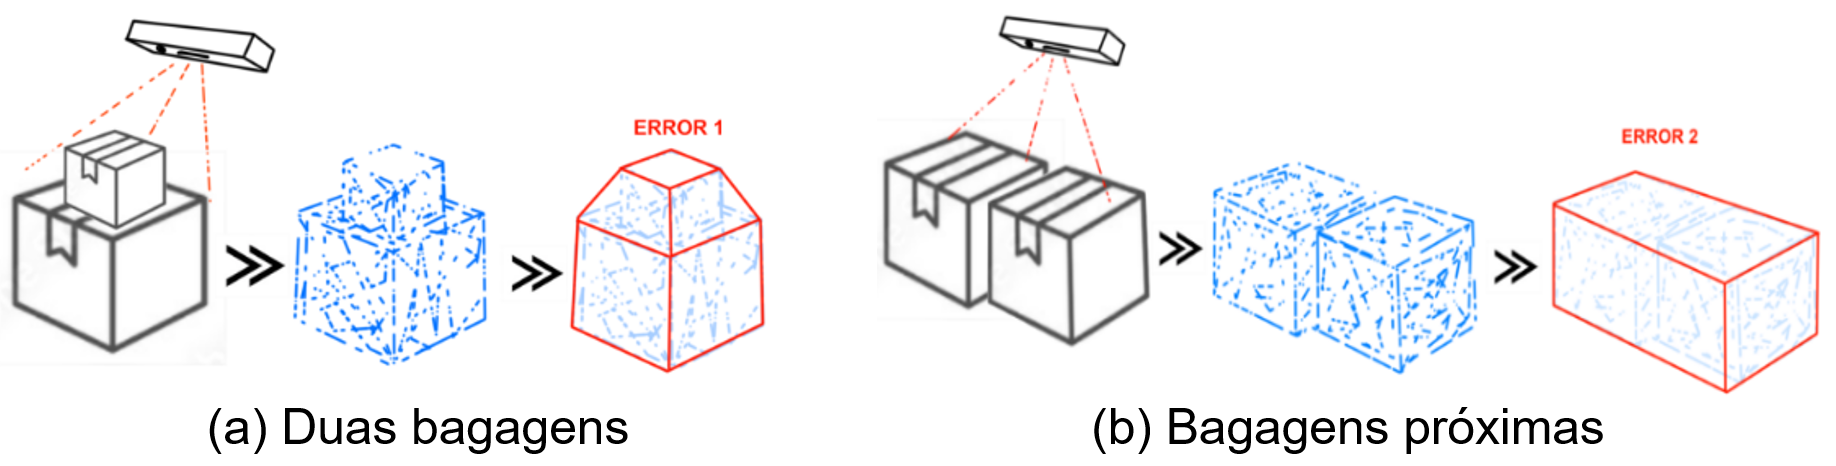
\includegraphics[width=0.9\textwidth]{imagens/PossiveisErrosComaisBagagens.png} 
           \caption{Possíveis erros ao lidar com mais de uma bagagem}
           \label{fig:PossiveisErrosComaisBagagens}
        \end{figure}

\subsection{Sensibilidade ao posicionamento da bagagem}
\label{subsec_Sensibilidade ao posicionamento da bagagem}


    Como analisado nos trabalhos, a posição do objeto alvo é comumente fixa em um único ângulo. Isso indica que aquele método foi especializado para tratar de objetos seguindo o mesmo padrão de posicionamento. Tais modelos podem gerar erros que ficam oclusos devido à posição ou forma do objeto. 
    
    Sobre este item, \citeonline{ozbay_2013_3d} destacam que houve perda de informações devido a não obtenção da \textit{point cloud} em 360°. Isso significa que se o objeto tiver alguma protuberância ou largura maior do lado ocluso, a amostra não coletaria essa informação, gerando erro. Em \citeonline{ruchay_2018_fusion}, por outro lado, esse problema é amenizado pelo uso de quatro kinects tendo o objeto posicionado ao centro do cenário de captura. Isso indica que existem casos onde é interessante ter duas ou mais perspectivas da \textit{point cloud} para analisar outras faces do objeto.


\subsection{Pontos em aberto}
\label{subsec_Pontos em aberto}

    Mediante a análise qualitativa dos trabalhos selecionados, é possível listar os seguintes problemas pendentes: 
    
    \begin{itemize}
        \item \textit{Reconstrução de múltiplos objetos}: exceto os estudos que utilizaram scanners a laser móveis, nenhum outro aplicou a reconstrução de múltiplos objetos do cotidiano ou bagagens (vide Figura \ref{fig:PossiveisErrosComaisBagagens}b que se baseia no método proposto com sensor de profundidade e ilustra duas situações onde são inseridos múltiplos objetos no self bag drop); 
        \item \textit{Flexibilidade e adaptabilidade}: Esse indicador significa que os trabalhos limitam tanto o cenário de teste quanto a complexidade do objeto. Vários estudos reconstruíram com fidelidade malas no formato cuboide, porém, foi possível identificar que os resultados são altamente influenciados pela posição, forma e quantidade das malas.
    \end{itemize}

    Considerando os pontos supracitados, os métodos empregados para identificar pontos alinhados poderiam ser aplicados na obtenção de dimensões de bagagens cuboides. No entanto, continuariam gerando erros nas detecções das dimensões de bagagens com deformações ou formatos não cuboides. Nesse caso, uma solução poderia ser complementar a análise com métodos que obtiveram dimensões de objetos utilizando espelhamento da \textit{point cloud}, conforme destacado na literatura e nos resultados. Já a clusterização pode ser utilizada para detectar as dimensões de múltiplas bagagens. Esse problema surge quando o cliente coloca duas ou mais malas de uma vez no equipamento, por conta da oclusão e do método poder retornar dados errôneos. Quanto à precisão do sistema, pôde ser notado que existe uma tolerância ao erro de medidas, o que indica que combinar esses métodos com sensores de profundidade pode ser uma boa alternativa para atingir um erro aceitável.
    
    Portanto, com base nos problemas supracitados, é possível afirmar que os principais desafios continuam ligados a capacidade de aplicabilidade em cenários não limitados, a complexidade do objeto, posicionamento e ao custo expressivo do equipamento. Também pode-se destacar que a utilização de mais de um método torna-se interessante para casos de malas com dimensões mais complexas, dados que podem ter grande valia para as companhias aéreas.

